%% 美赛模板:正文部分

\documentclass[12pt]{article}  % 官方要求字号不小于 12 号,此处选择 12 号字体
% 本模板不需要填写年份,以当前电脑时间自动生成
% 请在以下的方括号中填写队伍控制号
\usepackage[MI00008]{easymcm}  % 载入 EasyMCM 模板文件
\problem{A}  % 请在此处填写题号
% \usepackage{mathptmx}  % 这是 Times 字体,中规中矩 
\usepackage{mathpazo}  % 这是 COMAP 官方杂志采用的更好看的 Palatino 字体,可替代以上的 mathptmx 宏包
\title{An MCM Paper Made by Team MI00008}  % 标题
\usepackage{enumerate}
% 如需要修改题头(默认为 MCM/ICM),请使用以下命令(此处修改为 MCM)
%\renewcommand{\contest}{MCM}

% 文档开始
\begin{document}

% 此处填写摘要内容
\begin{abstract}
    Here is the abstract of your paper.
    Firstly, that is ...

    Secondly, that is ...

    Finally, that is ...

    % 美赛论文中无需注明关键字。若您一定要使用,
    % 请将以下两行的注释号 '%' 去除,以使其生效
    \vspace{5pt}
    \textbf{Keywords}: MATLAB, mathematics, LaTeX.

\end{abstract}

\maketitle  % 生成 Summary Sheet
\tableofcontents  % 生成目录


% 正文开始
\section{Introduction}
\subsection{Problem Background}
Here is the problem background ...
Two major problems are discussed in this paper, which are:
\begin{itemize}
    \item Doing the first thing.
    \item Doing the second thing.
\end{itemize}

\subsection{Literature Review}
A literatrue\cite{1} say something about this problem ...

\subsection{Our work}
We do such things ...

\begin{enumerate}[\bfseries 1.]
    \item We do ...
    \item We do ...
    \item We do ...
\end{enumerate}

\section{Preparation of the Models}
\subsection{Assumptions}

\subsection{Notations}
The primary notations used in this paper are listed in Table \ref{tb:notation}.

% 三线表示例
\begin{table}[!htbp]
\begin{center}
\caption{Notations}
\begin{tabular}{cl}
	\toprule
	\multicolumn{1}{m{3cm}}{\centering Symbol}
	&\multicolumn{1}{m{8cm}}{\centering Definition}\\
	\midrule
	$A$&the first one\\
	$b$&the second one\\
	$\alpha$ &the last one\\
	\bottomrule
\end{tabular}\label{tb:notation}
\end{center}
\end{table}

\section{The Models}
\subsection{Model 1}
\subsubsection{Details about Model 1}
The detail can be described by equation \eqref{eq:heat}:
\begin{equation}\label{eq:heat}
\frac{\partial u}{\partial t} - a^2 \left( \frac{\partial^2 u}{\partial x^2} + \frac{\partial^2 u}{\partial y^2} + \frac{\partial^2 u}{\partial z^2} \right) = f(x, y, z, t)
\end{equation}

\subsection{Model 2}
\subsubsection{Conclusion of Model 2}
The results are shown in Figure \ref{fig:result}, where $t$ denotes the time in seconds, and $c$ refers to the concentration of water in the boiler.

\begin{figure}[htbp]
\centering
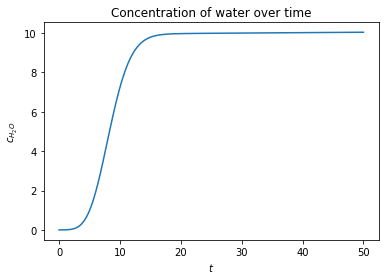
\includegraphics[width=.8\textwidth]{water.png}
\caption{The result of Model 2}\label{fig:result}
\end{figure}

\clearpage
\subsubsection{Commetary on Model 2}
The instance of long and wide tables are shown in Table \ref{tb:longtable}.

% 长表格示例,更多用法请参考 longtable 宏包文档
% 以下环境及对应参数可实现表格内的自动换行与表格的自动断页
% 您也可以选择自行载入 tabularx 宏包,并通过 X 参数指定对应列自动换行
\begin{longtable}{ p{4em} p{14em} p{14em} }
\caption{Basic Information about Three Main Continents (scratched from Wikipedia)}
\label{tb:longtable}\\
\toprule
Continent & Description & Information \\
\midrule
Africa & Africa Continent is surrounded by the Mediterranean Sea to the
north, the Isthmus of Suez and the Red Sea to the northeast, the Indian
Ocean to the southeast and the Atlantic Ocean to the west. &
At about 30.3 million km$^2$ including adjacent islands, it covers 6\%
of Earth's total surface area and 20\% of its land area. With 1.3
billion people as of 2018, it accounts for about 16\% of the world's
human population. \\
\midrule
Asia & Asia is Earth's largest and most populous continent which
located primarily in the Eastern and Northern Hemispheres.
It shares the continental landmass of Eurasia with the continent
of Europe and the continental landmass of Afro-Eurasia with both
Europe and Africa. &
Asia covers an area of 44,579,000 square kilometres, about 30\%
of Earth's total land area and 8.7\% of the Earth's total surface
area. Its 4.5 billion people (as of June 2019) constitute roughly
60\% of the world's population. \\
\midrule
Europe & Europe is a continent located entirely in the Northern
Hemisphere and mostly in the Eastern Hemisphere. It comprises the
westernmost part of Eurasia and is bordered by the Arctic Ocean to
the north, the Atlantic Ocean to the west, the Mediterranean Sea to
the south, and Asia to the east. &
Europe covers about 10,180,000 km$^2$, or 2\% of the Earth's surface
(6.8\% of land area), making it the second smallest
continent. Europe had a total population of about 741 million (about
11\% of the world population) as of 2018. \\
\bottomrule
\end{longtable}

Figure \ref{fig:subfigures} gives an example of subfigures. Figure \ref{subfig:left} is on the left, and Figure \ref{subfig:right} is on the right.

% 子图(多图并列)示例,更多用法请参考 subfigure 宏包文档
% 如果您只希望几张图并列,不需要额外的 caption,那么在 figure 环境中
% 连续插入总宽度不超过 \textwidth 的多个 \includegraphics 命令即可
\begin{figure}[htbp]
\centering
\begin{subfigure}[b]{.4\textwidth}
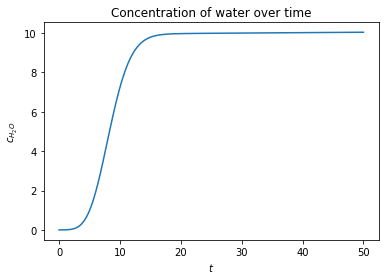
\includegraphics[width=\textwidth]{water.png}
\caption{Image on the left}\label{subfig:left}
\end{subfigure}
\begin{subfigure}[b]{.4\textwidth}
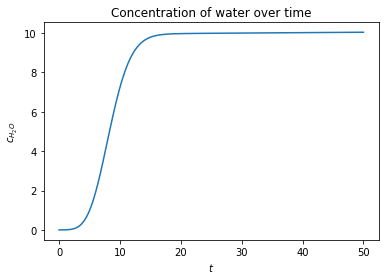
\includegraphics[width=\textwidth]{water.png}
\caption{Image on the right}\label{subfig:right}
\end{subfigure}
\caption{Two images}\label{fig:subfigures}
\end{figure}

\section{Strengths and Weaknesses}
\subsection{Strengths}
\begin{itemize}
    \item First one...
    \item Second one ...
\end{itemize}

\subsection{Weaknesses}
\begin{itemize}
    \item Only one ...
 \end{itemize}


\section{Establishment And Solution For Problem One}
\subsection{Selection of Indicators}
The early-warning mechanism of social security and stability refers to the critical state that signals the operation of society and shows that disorderly phenomena have taken place or are about to take place, a set of systems and methods aimed at attracting the attention of policy makers, managers and the public, analyzing the causes in a timely manner, and implementing effective measures so as to prevent the undesirable phenomena of social operation from further worsening. In the face of the rapid development of modern society, it will be helpful for government decision-making departments and public security organs to establish a complete and effective early-warning mechanism for social security and stability, guan took timely and effective preventive measures against risks in social development in order to maintain and promote social harmony and stability.

Social security is a more complex concept, and due to the broad nature of its content, there is a distinction between broad and narrow senses. Social security in the broadest sense refers to the state of social operation in which the entire social system can maintain benign operation and coordinated development, and the insecurity factors and influence are minimized. Obviously, social security includes economic security, political security, social life security, ideological and cultural security, and many other aspects. Social security in the narrow sense refers to security in areas other than economic and political systems. Based on the analysis of the above two aspects, we believe that the connotation of social security can be interpreted as: Social security refers to the security of the public living space of the population, which includes the security of citizens' lives and property, the order of social life, and the ecological environment, and it directly reflects the needs of public security interests closely related to citizens.

We believe that there is no absolute objectivity and reasonableness in the selection of indicators, of course, we cannot guarantee that the indicators we choose will be reasonable, but we read a lot of literature to ensure that our indicators are as objective and reasonable as possible within our ability.

Social stability includes political stability, economic stability, normal social order and people's peace of mind. These aspects are interrelated, mutually influencing, interacting and inseparable. Political stability is the core of social stability as a whole, economic stability is the foundation of social stability as a whole, normal social order is a necessary condition for political stability and economic stability, and people's peace of mind is a comprehensive reflection of social stability. We divide the indicators into three categories, police source indicators, warning indicators and alarm indicators. According to the analytic hierarchy method, the indicator system is divided into target layer($A_i$), criterion layer($A_{ij}$) and indicator layer($A_{ijk}$). The specific meaning of each of these indicators is listed in the Appendix A.

We have included our indicators in the following figure:
\begin{figure}[htbp]
\centering
\begin{subfigure}[b]{.32\textwidth}
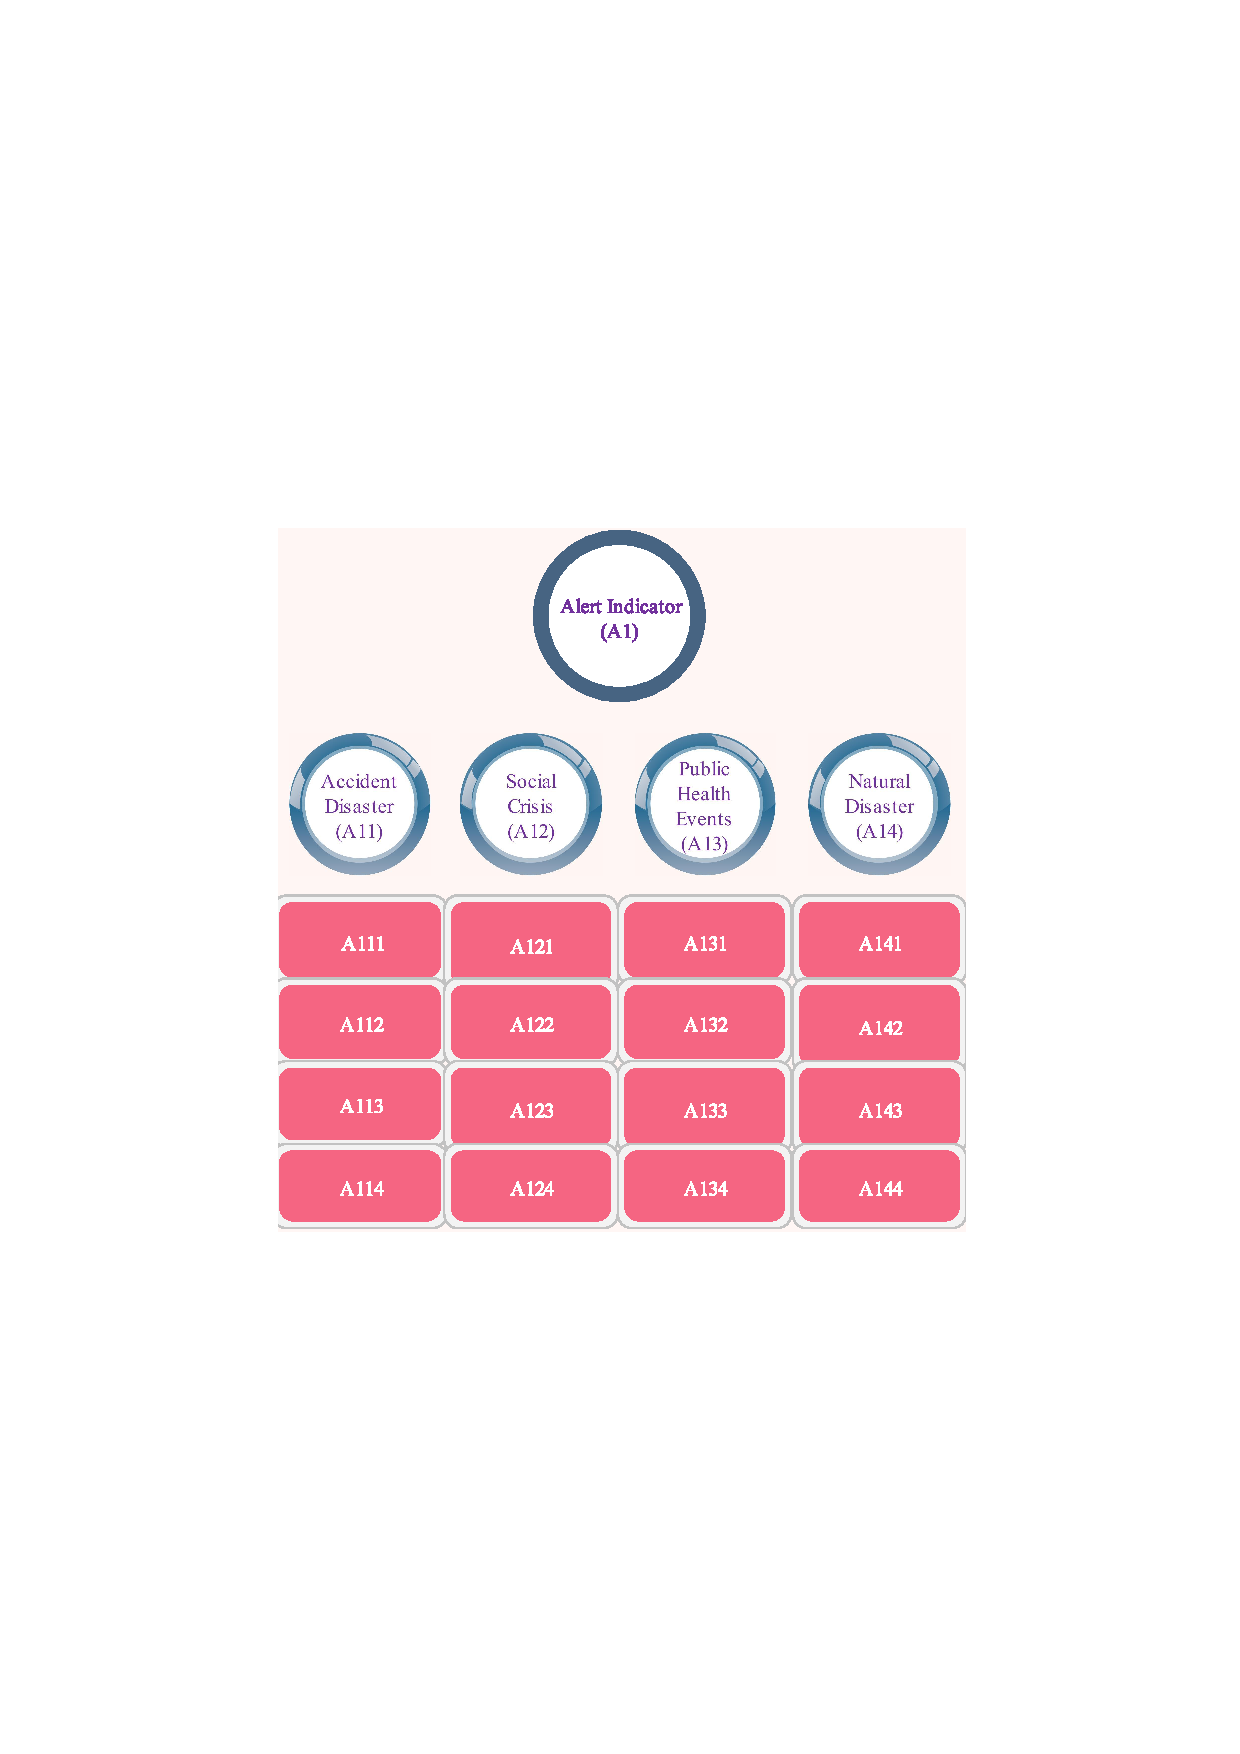
\includegraphics[width=\textwidth]{1}
\end{subfigure}
\begin{subfigure}[b]{.32\textwidth}
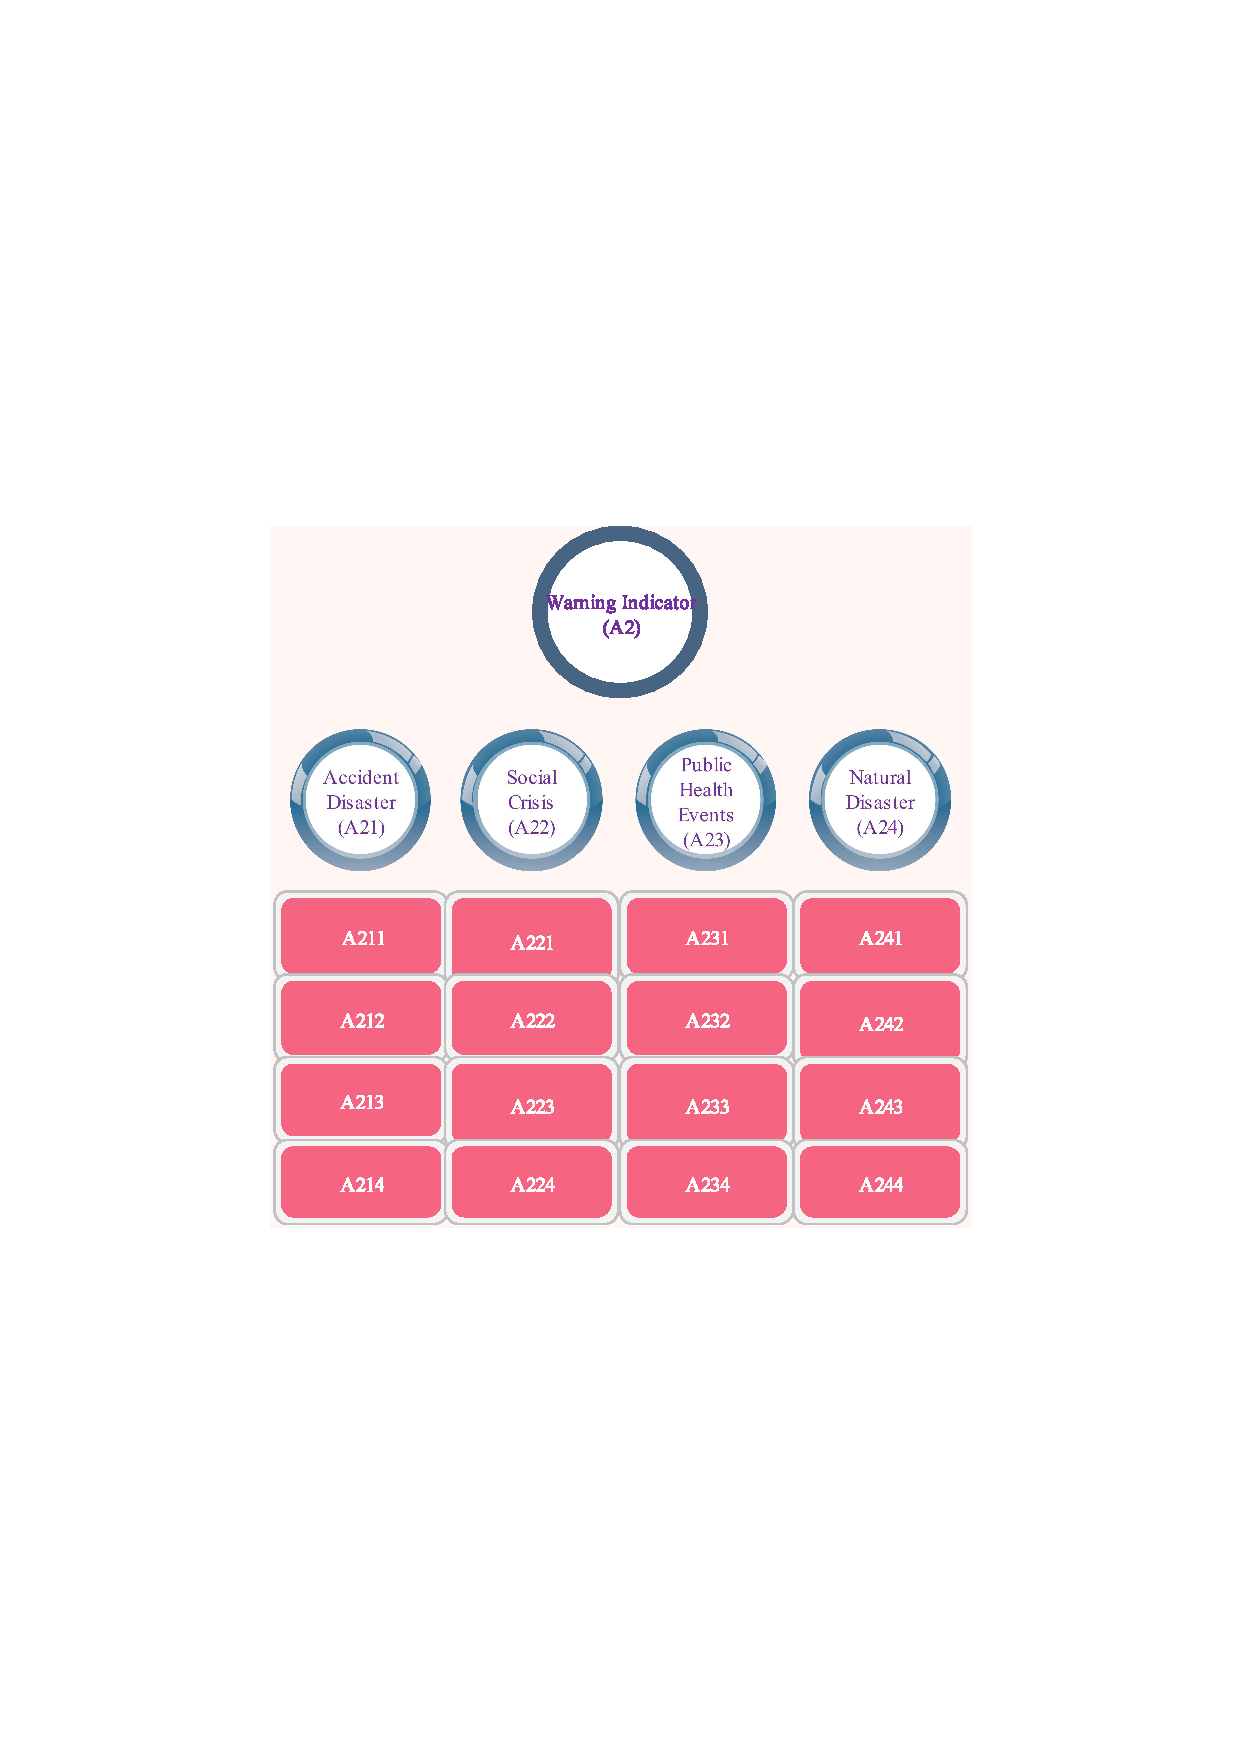
\includegraphics[width=\textwidth]{2}
\end{subfigure}
\begin{subfigure}[b]{.32\textwidth}
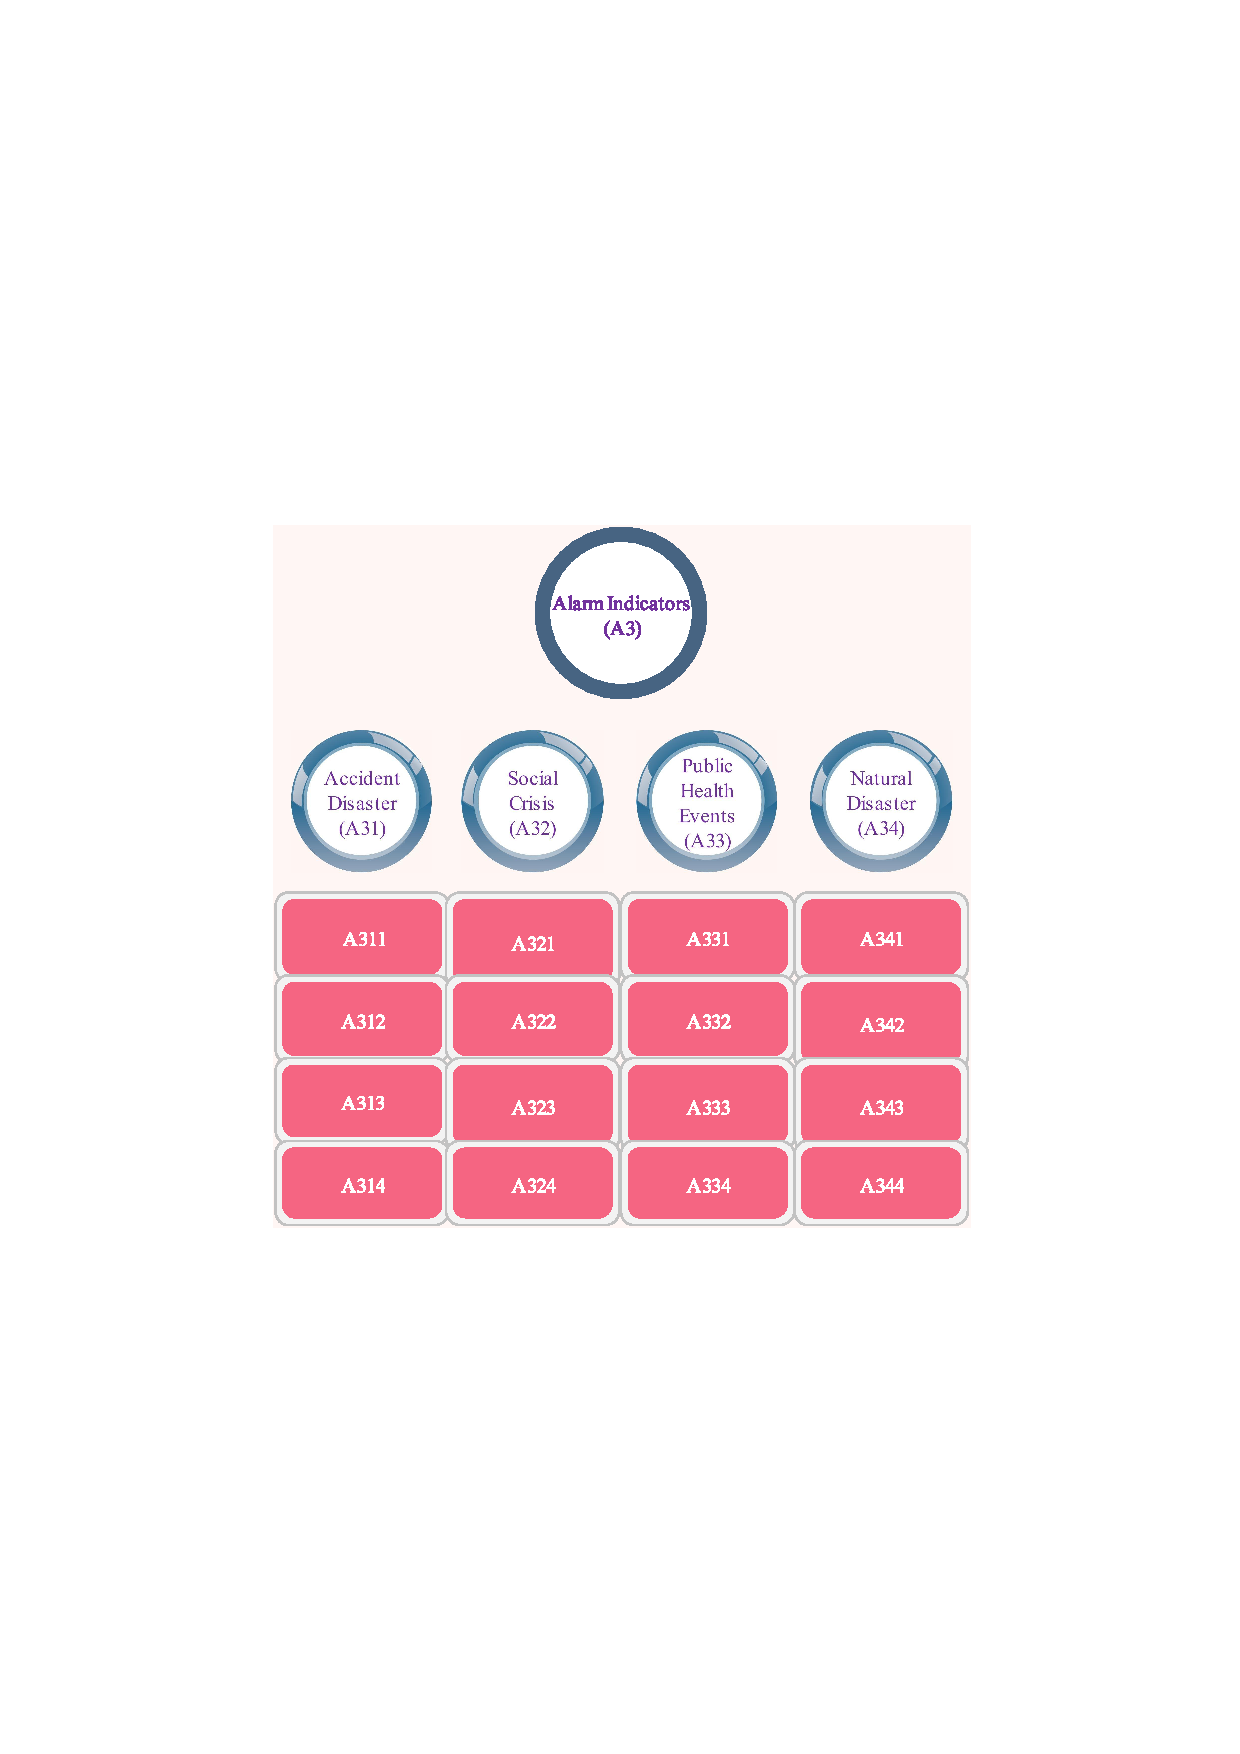
\includegraphics[width=\textwidth]{3}
\end{subfigure}
\caption{Selection of Indicators}
\end{figure}


































\subsection{Establishment of ISM Model}
ISM (Interpretive Structural Modeling) is a model that is developed to study complex systems. 
Based on tools such as directed graph, matrix and computer technology, a multi-level 
hierarchical structure model is constructed (POLAT \& RMAC, 2011, p. 169-174). DEMATEL 
(Decision Making Trial and Evaluation Lab), which is a scientific method based on graph theory 
and matrix to simplify the complex system structure (Gu Xuesong \& Chi Guotai, 2010, p. 508-
514). The combined model in this paper integrates the centrality and causation of DEMATEL 
into the multi-level hierarchical structure of ISM, which can not only clarify the hierarchical 
relationship of various influencing factors but also study the relative importance of constraints, 
so as to make the analysis result more objective and reasonable.
The steps to build the composite model are as follows:
\begin{enumerate}
    \renewcommand{\labelenumi}{\textbf{Step \theenumi}}
    \item Determine the set of influencing factors :
\begin{equation}
A=\{a_i|i=1,2,\cdots ,n\}
\end{equation}
    \item Determine the factor influence scale, and determine the mutual influence relationship between 
the factors through expert knowledge and experience, and get the direct influence matrix $V$.
\begin{equation}
    V=[v_{ij}]_{n\times n}
\end{equation}
Thereinto, $v_{ij}$ represents the influence degree of factor $a_i$ on factor $a_j$. When $i=j$ , $v_{ij}=0$.
    \item  Calculate the direct impact matrix $V$ to obtain the normalized direct impact matrix $X$ :
    \begin{equation}
X=[X_{ij}]_{n\times n}=\frac{V}{\max \sum_{j=1}^{n}V_{ij}}
\end{equation}
    \item Calculate the comprehensive impact matrix $T$ :
\begin{equation}
T=[T_{ij}]_{n\times n}=X(I-X)^{-1}
\end{equation}
Thereinto, $I$ is identity matrix.
    \item The influence degree $f_i$ , the influence degree $e_i$ , the center degree $z_i$ and the reason degree $y_i$ of 
the constraint factors were calculated. The calculation formula is as follows:
\begin{eqnarray}
    &f_i=\sum_{j=1}^{n}T_{ij},1\le i\le n \\
    &e_i=\sum_{j=1}^{n}T_{ij},1\le i\le n\\ 
    &z_i=f_i+e_i\\
    &y_i=f_i-e_i
\end{eqnarray}
    \item Draw the cause and result diagram:

Cartesian coordinate system is drawn with the degree of center as the abscissa and the degree of 
cause as the ordinate.
    \item  Calculate the overall impact matrix $H$ :
    \begin{equation}
        H=[H_{ij}]_{n\times n}=T+I
    \end{equation}
    \item Determine the threshold value $\lambda$ (Xue Wei1 \& Geng Zhiwei, et al. 2019, p. 99-104.):
\begin{equation}
    \lambda =\alpha +\beta
\end{equation}
Where, and respectively refer to the mean value and standard deviation of the comprehensive 
influence matrix $T$ .Different $\lambda$ values have different logical relationships with the 
influencing factors (Sun Jing, 2018). The choice of $\lambda$ is more subjective based on expert 
experience, while replacing it with the sum of the mean and standard deviation based on the 
statistical distribution is more objective, which can reduce the influence of subjectivity.
    \item Calculate the standardized reachable matrix $K$ :
\begin{equation}
    K=[K_{ij}]_{n\times n}
\end{equation}
Thereinto, if $H_{ij}>\lambda$ ,then $H_{ij}=1$ 

\hspace{4.5em} if $H_{ij}\le \lambda$ ,then $H_{ij}=0$ .
\item  According to the reachability matrix, the reachability set $R_i$ and antecedent set $S_i$ of each 
influencing factor are determined.\\ 
Thereinto, $R_i$ is composed of the index set corresponding to all the 
columns with index 1 in the ith row of the reachable matrix

\hspace{4.5em} $S_i$ consists of the set of indices 
corresponding to all rows with index 1 in the ith column of the reachable matrix.
\item Verify:
\begin{equation}
    R_i=R_i\cap S_i,(i=1,2,\cdots ,n)
\end{equation}
If it is true, then $a_i$ is the highest level factor. At this time, row $i$ and column $i$ are deleted in $K$ , 
and the calculation is repeated until all factors are deleted.
\item Draw the hierarchical structure diagram of factors according to the order of factors to be 
deleted, and establish the structural model.
\end{enumerate}






















% 以下为信件/备忘录部分,不需要可自行去掉
% 如有需要可将整个 letter 环境移动到文章开头或中间
% 请在第二个花括号内填写标题,如「信件」(Letter)或「备忘录」(Memorandum)
\begin{letter}{Memorandum}
\begin{flushleft}  % 左对齐环境,无首行缩进
\textbf{To:} Heishan Yan\\
\textbf{From:} Team 1234567\\
\textbf{Date:} October 1st, 2019\\
\textbf{Subject:} A better choice than MS Word: \LaTeX
\end{flushleft}

In the memo, we want to introduce you an alternate typesetting program to the prevailing MS Word: \textbf{\LaTeX}. In fact, the history of \LaTeX\ is even longer than that of MS Word. In 1970s, the famous computer scientist Donald Knuth first came out with a typesetting program, which named \TeX\ \ldots

Firstly, \ldots

Secondly, \ldots

Lastly, \ldots

According to all those mentioned above, it is really worth to have a try on \LaTeX! 
\end{letter}


% 参考文献,此处以 MLA 引用格式为例
\begin{thebibliography}{99}
\bibitem{1} Einstein, A., Podolsky, B., \& Rosen, N. (1935). Can quantum-mechanical description of physical reality be considered complete?. \emph{Physical review}, 47(10), 777.
\bibitem{2} \emph{A simple, easy \LaTeX\ template for MCM/ICM: EasyMCM}. (2018). Retrieved December 1, 2019, from\url{https://www.cnblogs.com/xjtu-blacksmith/p/easymcm.html}
\end{thebibliography}


% 以下为附录内容
% 如您的论文中不需要附录,请自行删除
\begin{subappendices}  % 附录环境
\section{Appendix A: Specific Meanings of Indicators}
\label{a1}
To clarify the importance of using \LaTeX\ in MCM or ICM, several points need to be covered, which are \ldots

To be more specific, \ldots

All in all, \ldots

Anyway, nobody \textbf{really} needs such appendix \ldots

\section{Appendix B: Program Codes}
Here are the program codes we used in our research.

% 代码环境示例三则
% 如您的论文不需要展示代码,请删除
% 更多用法,请参考 listings 宏包文档

% Python 代码示例
\begin{lstlisting}[language=Python, name={test.py}]
# Python code example
for i in range(10):
    print('Hello, world!')
\end{lstlisting}

% MATLAB 代码示例
\begin{lstlisting}[language=MATLAB, name={test.m}]
% MATLAB code example
for i = 1:10
    disp("hello, world!");
end
\end{lstlisting}

% C++ 代码示例
\begin{lstlisting}[language=C++, name={test.cpp}]
// C++ code example
#include <iostream>
using namespace std;

int main() {
    for (int i = 0; i < 10; i++)
        cout << "hello, world" << endl;
    return 0;
}
\end{lstlisting}

\end{subappendices}  % 附录内容结束

\end{document}  % 结束
